\documentclass[aspectratio=169,11pt]{beamer}

% Shared style (ib-tutorials.sty at the repo root).
\makeatletter\def\input@path{{./}{../}}\makeatother
\usepackage{ib-tutorials}

\usepackage[utf8]{inputenc}
\usepackage{amsmath,amssymb}
\usepackage{booktabs}
\usepackage{array}
\newcolumntype{L}[1]{>{\raggedright\arraybackslash}p{#1}}
\usepackage{graphicx}
\graphicspath{{../pictures/3-ibamr-fundamentals/}{pictures/3-ibamr-fundamentals/}}
\usepackage{xcolor}
\usepackage{listings}
\usepackage{tikz}
\usetikzlibrary{arrows.meta,positioning,shapes.geometric,fit,calc}
\usepackage{hyperref}

\newcommand{\sourcecredit}[1]{\vfill\hfill{\tiny\textcolor{DarkGray}{#1}}}

\lstset{
  basicstyle=\ttfamily\scriptsize\color{BlackGray},
  keywordstyle=\color{NavyBlue}\bfseries,
  commentstyle=\color{DarkGray}\itshape,
  stringstyle=\color{OliveGreen},
  showstringspaces=false,
  columns=fullflexible,
  keepspaces=true,
  frame=single,
  framerule=0.4pt,
  rulecolor=\color{LightGray},
  backgroundcolor=\color{LightGray!30},
  xleftmargin=0.25em,
  xrightmargin=0.25em
}
\lstdefinestyle{shell}{morecomment=[l]{\#}}
\lstdefinestyle{input}{morecomment=[l]{//}}
\lstdefinestyle{matlab}{morecomment=[l]{\%}}

\title[The IB method]{The immersed boundary method and numerical considerations}
\subtitle{What IBAMR solves, how it couples the fluid to the structure, and why runs blow up}
\author[Miller]{Laura A. Miller}
\institute[UArizona]{Department of Mathematics, University of Arizona}
\date{Using IB Software \textbullet\ Part III \textbullet\ Chapter 5}

% a small Eulerian grid with a Lagrangian curve and one point's stencil
\newcommand{\ibpicture}[1]{%
\begin{tikzpicture}[scale=#1]
  \draw[LightGray!80,step=1] (0,0) grid (8,8);
  \fill[RubineRed!18] (3,3) rectangle (7,7);
  \draw[RubineRed,thick] (4.6,5.3) node[circle,fill=RubineRed,inner sep=1.4pt] {} node[above right,font=\tiny,text=RubineRed] {$X(q)$};
  \draw[NavyBlue,very thick] plot[smooth] coordinates {(1,1.2) (2.5,2.6) (4.6,5.3) (6.2,6.4) (7.6,7.4)};
  \node[font=\tiny,text=NavyBlue] at (2.4,3.6) {structure $X(q,t)$};
  \node[font=\tiny,text=DarkGray] at (6.6,1.2) {fluid grid $u(x,t)$};
  \node[font=\tiny,text=RubineRed] at (5,2.5) {$4\times4$ cells share the point's force};
\end{tikzpicture}}

\begin{document}

% 1
\begin{frame}[plain]
\maketutorialtitlepanel{\ibpicture{0.6}}
\end{frame}

% 2
\begin{frame}{Learning goals}
By the end of this chapter you should be able to:
\begin{enumerate}
  \item write down the equations that an IB simulation solves and say what each term does;
  \item explain how the fluid grid and the structure talk to each other through regularized delta functions, and what that implies for point spacing and the thickness of a boundary;
  \item use the words convergence, order and stability correctly, and show each with the two demo scripts;
  \item say what limits the time step in an IB simulation and read the error IBAMR prints when the limit is crossed;
  \item explain what adaptive mesh refinement does in IBAMR and which input keys control the time step, the grid and the coupling.
\end{enumerate}
\vspace{3mm}
\begin{punchbox}
\small This chapter is the practical overview. The derivations are in the companion series \emph{Fluid Dynamics and IBM Theory}, modules 0-1 (Navier--Stokes), 0-2 (non-dimensionalization) and 1-1 to 1-4 (the IB method, its formulation, the integral transforms and the discretization).
\end{punchbox}
\end{frame}

% 3
\begin{frame}{Fluid--structure interaction in biology}
\begin{columns}[T,onlytextwidth]
\begin{column}{0.55\textwidth}
Organisms move fluid and are moved by it, from the heart of a whale to a swimming bacterium. The same equations hold; what changes is the balance between inertia and viscosity, the Reynolds number.
\scriptsize
\begin{tabular}{@{}L{0.28\linewidth}L{0.31\linewidth}L{0.29\linewidth}@{}}
\toprule
Regime & Examples in the old lectures & Examples in this series\\
\midrule
High Re: inertia matters & the whale heart (a chambered pump); the stingray (flapping locomotion) & jellyfish bells, insect wings, the flow tank (IBFE/10)\\
Low Re: viscosity dominates & cilia in the respiratory tract (micropumps); \emph{E.\ coli} (flagellar locomotion) & bristled wings (IB/04), the glycocalyx (IB/08), heart tubes\\
\bottomrule
\end{tabular}
\end{column}
\begin{column}{0.43\textwidth}
\begin{punchbox}
\small The immersed boundary method handles both regimes with one code: an elastic structure in a viscous incompressible fluid, on a fixed grid. That is why one tutorial covers whale hearts and bacteria.
\end{punchbox}
\vspace{2mm}
\small The 2014--2025 lectures opened with four photographs of these organisms; they were third-party images and are replaced here by the table.
\end{column}
\end{columns}
\end{frame}

% 4
\begin{frame}{Modeling the fluid: the Navier--Stokes equations}
For a viscous, incompressible fluid with velocity $\mathbf{u}(\mathbf{x},t)$ and pressure $p(\mathbf{x},t)$,
\begin{align*}
\rho\left(\frac{\partial \mathbf{u}}{\partial t} + \mathbf{u}\cdot\nabla\mathbf{u}\right) &= -\nabla p + \mu\,\Delta\mathbf{u} + \mathbf{f}, \\
\nabla\cdot\mathbf{u} &= 0 .
\end{align*}
\begin{columns}[T,onlytextwidth]
\begin{column}{0.55\textwidth}
\small
\begin{itemize}
  \item The first line is Newton's second law, $F = ma$, for a parcel of fluid: mass per volume $\rho$ times acceleration equals the forces per volume.
  \item $-\nabla p$: the pressure pushes from high to low; $\mu\Delta\mathbf{u}$: viscosity smooths velocity differences; $\mathbf{f}$: the force per volume that the \al{immersed structure} puts on the fluid.
  \item The second line says the fluid is incompressible: what flows into a region flows out.
\end{itemize}
\end{column}
\begin{column}{0.43\textwidth}
\begin{punchbox}
\small $\rho$ is the density and $\mu$ the (dynamic) viscosity: in \code{input2d} they are \code{RHO} and \code{MU}. In the IB examples they are in SI units (1000 kg/m$^3$ and 100 N\,s/m$^2$ for the rubber band); in the IBFE examples they are dimensionless.
\end{punchbox}
\vspace{1mm}
\small Derivation: \emph{Theory}, module 0-1.
\end{column}
\end{columns}
\end{frame}

% 5
\begin{frame}{The non-dimensional form}
Choose a characteristic length $L$ (the length of a wing) and velocity $V$ (the speed of the wing tip), and write $\mathbf{x} = L\,\mathbf{x}'$, $\mathbf{u} = V\mathbf{u}'$, $t = (L/V)\,t'$, $p = \rho V^2 p'$. Then
\[
\frac{\partial \mathbf{u}'}{\partial t'} + \mathbf{u}'\cdot\nabla'\mathbf{u}' = -\nabla' p' + \frac{1}{Re}\,\Delta'\mathbf{u}' + \mathbf{f}', \qquad Re = \frac{\rho V L}{\mu}.
\]
\begin{columns}[T,onlytextwidth]
\begin{column}{0.55\textwidth}
\begin{itemize}
  \item One number, the \al{Reynolds number}, is left: the ratio of inertial to viscous forces.
  \item Everything else (density, viscosity, size, speed) enters only through $Re$ and through the dimensionless force $\mathbf{f}' = \mathbf{f} L/(\rho V^2)$.
  \item IBAMR does not care whether your input is in meters and seconds or dimensionless, as long as every number is in the same system. Chapter 8b shows how to convert a model.
\end{itemize}
\end{column}
\begin{column}{0.43\textwidth}
\begin{punchbox}
\small A choice to make early: the IB examples here keep SI units because the structure files were written that way; the IBFE examples are dimensionless because IBAMR's own examples are. Mixing them is the most common way to get a Reynolds number wrong by a factor of a thousand.
\end{punchbox}
\vspace{1mm}
\small Derivation: \emph{Theory}, module 0-2.
\end{column}
\end{columns}
\end{frame}

% 6
\begin{frame}{The Reynolds number}
\begin{columns}[T,onlytextwidth]
\begin{column}{0.55\textwidth}
\begin{itemize}
  \item Flows with the same $Re$ (and the same geometry and boundary conditions) are \al{dynamically similar}: the same dimensionless velocity field, the same force coefficients.
  \item That is how physical models work: a larger model of a small organism in a more viscous fluid (glycerin, oil), or a smaller, faster model of a large one.
  \item In a simulation the same freedom exists: a bristled wing a thousand times larger than the insect's, in a fluid a thousand times more viscous, gives the same flow. Use it to keep numbers near 1.
\end{itemize}
\end{column}
\begin{column}{0.43\textwidth}
\scriptsize
\begin{tabular}{@{}L{0.42\linewidth}L{0.48\linewidth}@{}}
\toprule
Example & $Re$ and how it is built\\
\midrule
IB/01 rubber band & very low ($\mu = 100$, $\rho = 1000$, $V\sim0.1$, $L = 0.2$: $Re \approx 0.2$)\\
IB/03 tethered leaf & $\rho V \ell/\mu = 2.5$\\
IB/04 bristles & 0.01 per bristle, 0.8 for the row\\
IB/08 glycocalyx (3D) & 0.06\\
IBFE/10 flow tank (3D) & 20 (speed 0.1, width 2, $\mu = 0.01$)\\
\bottomrule
\end{tabular}
\vspace{2mm}
\begin{punchbox}
\small Chapter 1b gave the comfortable ranges: IB2d up to about $10^3$, IBAMR up to a few $10^3$. Above that the boundary layers are thinner than the grid resolves, and the cost grows fast.
\end{punchbox}
\end{column}
\end{columns}
\end{frame}

% 7
\begin{frame}{Describing the structure}
\begin{columns}[T,onlytextwidth]
\begin{column}{0.55\textwidth}
In the immersed boundary method the structure is \al{always elastic}:
\begin{itemize}
  \item it can be stiff enough to act like a rigid object, but it is still a collection of elastic elements;
  \item it can be moved in prescribed ways with \al{target points}, stiff springs between the structure and a path you choose (chapter 9a);
  \item it can resist stretching (springs), bending (beams), and twisting (rods), and it can carry mass (chapter 13);
  \item every one of these properties can change in time, by a formula or by another model (muscle activation, growth: chapters 9b and 20).
\end{itemize}
\end{column}
\begin{column}{0.43\textwidth}
\begin{punchbox}
\small In IBAMR the structure is a list of points in a \code{.vertex} file and lists of elements that join them: \code{.spring}, \code{.beam}, \code{.target}, \ldots\ (chapter 6). In IBFE it is a finite element mesh with a material model (Part IV). Both produce the same thing the fluid needs: a force at every point.
\end{punchbox}
\end{column}
\end{columns}
\end{frame}

% 8
\begin{frame}{The immersed boundary idea}
\begin{columns}[T,onlytextwidth]
\begin{column}{0.48\textwidth}
\centering\ibpicture{0.5}
\end{column}
\begin{column}{0.5\textwidth}
Two descriptions, one problem:
\begin{itemize}
  \item \al{Eulerian}: the fluid lives on a fixed Cartesian grid. Unknowns at the grid points: velocity $\mathbf{u}(\mathbf{x},t)$, pressure $p(\mathbf{x},t)$, and the force density $\mathbf{f}(\mathbf{x},t)$ that the structure exerts.
  \item \al{Lagrangian}: the structure is a curvilinear mesh of material points labelled by $q$. Unknowns on the mesh: position $\mathbf{X}(q,t)$ and elastic force density $\mathbf{F}(q,t)$.
\end{itemize}
\end{column}
\end{columns}
\end{frame}

% 8b
\begin{frame}{The immersed boundary idea: what the fixed grid buys}
\begin{itemize}
  \item The grid does \emph{not} follow the structure, and the structure does not know about the grid. Each is discretized where it lives, and the two are coupled by integrals with delta functions.
  \item A body-fitted method would rebuild its mesh every time the structure moved; a jellyfish bell that folds, a heart valve that closes, or two wings that touch would each be a meshing problem of its own. Here the structure can do anything, including crossing itself, and the grid never changes.
  \item The structure can also be anything from a single point to a finite element solid; it only has to produce a force at each of its points.
\end{itemize}
\vspace{2mm}
\begin{punchbox}
\small No body-fitted mesh, no remeshing when the structure moves: that is the whole point, and the price is a boundary a few cells thick (slide 16).
\end{punchbox}
\end{frame}

% 9
\begin{frame}{One time step}
\begin{columns}[T,onlytextwidth]
\begin{column}{0.5\textwidth}
\centering
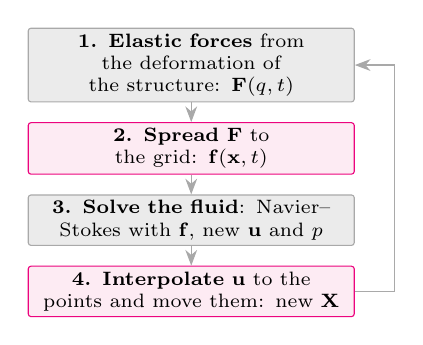
\begin{tikzpicture}[node distance=2.5mm and 6mm]
  \node[draw=DarkGray,rounded corners=1pt,fill=LightGray!45,text width=40mm,align=center,inner sep=2pt,font=\scriptsize] (a) {\textbf{1. Elastic forces} from the deformation of the structure: $\mathbf{F}(q,t)$};
  \node[draw=RubineRed,rounded corners=1pt,fill=RubineRed!8,text width=40mm,align=center,inner sep=2pt,font=\scriptsize,below=of a] (b) {\textbf{2. Spread} $\mathbf{F}$ to the grid: $\mathbf{f}(\mathbf{x},t)$};
  \node[draw=DarkGray,rounded corners=1pt,fill=LightGray!45,text width=40mm,align=center,inner sep=2pt,font=\scriptsize,below=of b] (c) {\textbf{3. Solve the fluid}: Navier--Stokes with $\mathbf{f}$, new $\mathbf{u}$ and $p$};
  \node[draw=RubineRed,rounded corners=1pt,fill=RubineRed!8,text width=40mm,align=center,inner sep=2pt,font=\scriptsize,below=of c] (d) {\textbf{4. Interpolate} $\mathbf{u}$ to the points and move them: new $\mathbf{X}$};
  \foreach \p/\q in {a/b,b/c,c/d} \draw[-{Stealth[length=2mm]},DarkGray] (\p) -- (\q);
  \draw[-{Stealth[length=2mm]},DarkGray] (d.east) -- ++(5mm,0) |- (a.east);
\end{tikzpicture}
\end{column}
\begin{column}{0.48\textwidth}
\footnotesize
\begin{itemize}
  \item Steps 1 and 4 happen on the structure, step 3 on the grid, and steps 2 and 4 are the \al{coupling}: the same regularized delta function spreads forces one way and interpolates velocities the other.
  \item Step 4 says that the structure moves with the fluid: the no-slip condition, enforced by construction.
  \item IBAMR's default scheme evaluates the forces and the velocity at the half step (the midpoint rule), which makes the coupling second-order accurate in time (slide 26).
\end{itemize}
\begin{punchbox}
\small The screen output of every example shows this loop: \code{At beginning of timestep}, the fluid solve's residuals, \code{integral\{F\}} (the sum of the spread forces), \code{At end of timestep}.
\end{punchbox}
\end{column}
\end{columns}
\end{frame}

% 10
\begin{frame}{The IB equations}
The Navier--Stokes equations with the structure's force, plus two coupling equations and an elasticity law:
\begin{align*}
\rho\left(\mathbf{u}_t + \mathbf{u}\cdot\nabla\mathbf{u}\right) &= -\nabla p + \mu\Delta\mathbf{u} + \mathbf{f}, \qquad \nabla\cdot\mathbf{u} = 0,\\
\mathbf{f}(\mathbf{x},t) &= \int_\Omega \mathbf{F}(q,t)\,\delta\big(\mathbf{x} - \mathbf{X}(q,t)\big)\,dq, \\
\frac{\partial \mathbf{X}}{\partial t}(q,t) &= \mathbf{u}\big(\mathbf{X}(q,t),t\big) = \int \mathbf{u}(\mathbf{x},t)\,\delta\big(\mathbf{x}-\mathbf{X}(q,t)\big)\,d\mathbf{x}, \\
\mathbf{F}(q,t) &= \mathcal{F}\big[\mathbf{X}(\cdot,t)\big](q) .
\end{align*}
\small Here $\mathbf{x}$ are the fixed physical coordinates, $q$ the material coordinate of the structure (its arc length, say), $\Omega$ the set of material coordinates, and $\delta$ the Dirac delta function (in 2D, $\delta(x)\delta(y)$). \emph{Theory}, modules 1-2 and 1-3, derive these equations and show that the transforms conserve total force and torque.
\end{frame}

% 10b
\begin{frame}{The IB equations, line by line}
\begin{itemize}
  \item \al{The first line} is the Navier--Stokes system of slide 4 with one addition: the force density $\mathbf{f}$ that the structure exerts on the fluid. The fluid does not know what the structure is, only where it pushes.
  \item \al{The second line} converts the Lagrangian force density $\mathbf{F}$ (force per unit $q$, defined on the structure) into an Eulerian force density $\mathbf{f}$ (force per unit area or volume, defined on the grid): a point at $\mathbf{X}(q,t)$ puts its force at that position and nowhere else.
  \item \al{The third line} is the no-slip condition: each material point moves at the fluid velocity where it is. Written as an integral with the same $\delta$, it is the transpose of the second line.
  \item \al{The last line} is the elasticity: $\mathbf{F}$ depends on the whole configuration $\mathbf{X}(\cdot,t)$, through springs, beams and target points (chapters 6, 9 and 10) or through a finite element stress (Part IV). It is the only line you write yourself.
\end{itemize}
\end{frame}

% 11
\begin{frame}{What the delta functions mean}
\begin{columns}[T,onlytextwidth]
\begin{column}{0.55\textwidth}
\small Integrate the force equation over any region $R$ of the fluid:
\[
\int_R \mathbf{f}\,d\mathbf{x} = \int_\Omega \mathbf{F}(q,t)\,\underbrace{\int_R \delta\big(\mathbf{x}-\mathbf{X}(q,t)\big)\,d\mathbf{x}}_{1 \text{ if } \mathbf{X}(q,t)\in R,\ 0 \text{ otherwise}}\,dq ,
\]
so the force on the fluid in $R$ is exactly the sum of the elastic forces of the material points that lie in $R$. Nothing is lost or created: the structure's force is simply handed to the fluid where the structure is.
\vspace{1mm}

The velocity equation reads the other way: the velocity of material point $q$ is the fluid velocity at its position, $\mathbf{u}(\mathbf{X}(q,t),t)$. Writing it as an integral with the same $\delta$ is what lets the discrete version use the same kernel for both directions.
\end{column}
\begin{column}{0.43\textwidth}
\begin{punchbox}
\small Using the \emph{same} regularized delta function for spreading and interpolation is not a convenience: it is what makes the discrete coupling conserve energy, so that the elastic energy stored in the structure equals the work done on the fluid. Peskin (2002) explains why.
\end{punchbox}
\end{column}
\end{columns}
\end{frame}

% 12
\begin{frame}{Spreading the force to the grid}
\begin{columns}[T,onlytextwidth]
\begin{column}{0.46\textwidth}
\centering\ibpicture{0.45}
\end{column}
\begin{column}{0.52\textwidth}
\small On the grid, with cell size $h$ and points $\mathbf{X}_k$ carrying forces $\mathbf{F}_k$ (force per unit $q$, times the spacing $\Delta q$):
\[
\mathbf{f}(\mathbf{x}_{ij}) = \sum_k \mathbf{F}_k\, \delta_h(\mathbf{x}_{ij} - \mathbf{X}_k)\,\Delta q ,
\]
with the \al{regularized} delta function $\delta_h(\mathbf{x}) = \frac{1}{h^2}\phi\!\left(\frac{x}{h}\right)\phi\!\left(\frac{y}{h}\right)$ (and a third factor in 3D).
\begin{itemize}
  \item $\phi$ is zero beyond a few cells, so each point's force lands on a small block of cells around it: $4\times4$ for the 4-point kernel, with weights that add up to 1.
  \item A boundary that resists bending or stretching produces forces along it; the picture shows one point's share of the grid.
\end{itemize}
\end{column}
\end{columns}
\end{frame}

% 13
\begin{frame}{Interpolating the velocity to the points}
\begin{columns}[T,onlytextwidth]
\begin{column}{0.48\textwidth}
\small The velocity of point $k$ is the weighted sum of the velocities of the same block of cells:
\[
\mathbf{U}_k = \sum_{ij} \mathbf{u}(\mathbf{x}_{ij})\,\delta_h(\mathbf{x}_{ij} - \mathbf{X}_k)\,h^2 ,
\]
and the point moves with it: $\mathbf{X}_k^{n+1} = \mathbf{X}_k^n + \Delta t\,\mathbf{U}_k$ (with the midpoint rule, the velocity at the half step).
\begin{itemize}
  \item The weights are the kernel evaluated at the distance from the cell to the point, in cells; at a given step the velocity in every cell is known.
  \item The same $\phi$, the same block of cells: the transpose of the spreading operation.
\end{itemize}
\end{column}
\begin{column}{0.5\textwidth}
\begin{punchbox}
\small Because the velocity is interpolated from a block of cells, a point never sees a velocity jump: the boundary is \emph{smeared} over the kernel's width. Two surfaces closer than that width share the same fluid cells and cannot be told apart by the fluid (slide 16).
\end{punchbox}
\vspace{2mm}
\small On an adaptive grid the points always live on the finest level, so $h$ here is the finest cell size, $\Delta x = L/N_{\text{finest}}$ in the input files (slides 32--33).
\end{column}
\end{columns}
\end{frame}

% 14
\begin{frame}{Regularized delta functions}
\small Peskin's 4-point kernel, \code{IB\_4}, is
\[
\phi(r) = \begin{cases}
\frac{1}{8}\big(3 - 2|r| + \sqrt{1 + 4|r| - 4r^2}\big), & |r| \le 1,\\[2pt]
\frac{1}{8}\big(5 - 2|r| - \sqrt{-7 + 12|r| - 4r^2}\big), & 1 \le |r| \le 2,\\[2pt]
0, & |r| \ge 2 .
\end{cases}
\]
\centering
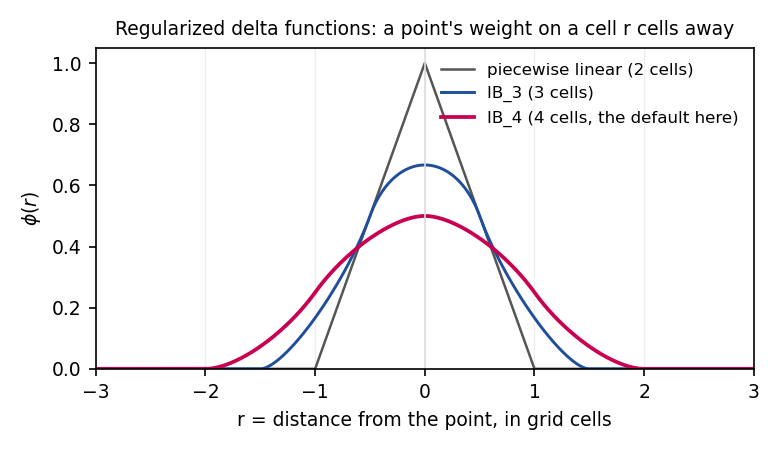
\includegraphics[width=0.62\linewidth]{ch5-delta-kernels.png}
\end{frame}

% 14b
\begin{frame}{What a kernel must satisfy}
\small What a kernel $\phi$ should satisfy, and why:
\begin{itemize}
  \item \al{continuous}, so that a point moving smoothly across the grid feels a smoothly changing velocity and exerts a smoothly changing force;
  \item \al{bounded support} (a few cells), so that each point touches only its neighborhood and the sums on slides 12 and 13 are cheap;
  \item the \al{discrete moment conditions}: $\sum_j \phi(r - j) = 1$ and $\sum_j (r-j)\,\phi(r-j) = 0$ for every $r$, so that total force and torque are conserved whatever the point's position relative to the grid;
  \item a constraint that makes the result nearly \al{independent of where the point sits} relative to the grid ($\sum_j \phi(r-j)^2$ constant), so that a structure does not feel the grid lines as it moves;
  \item for the 4-point kernel, the extra condition that the even and the odd grid points each receive half the weight, which lets it work with the staggered grid.
\end{itemize}
\vspace{2mm}
\begin{punchbox}
\small Peskin (2002), section 6, derives \code{IB\_4} from exactly these conditions; \emph{Theory}, module 1-3, works through it. The figure on the previous slide is plotted from the formulas, with IBAMR's names.
\end{punchbox}
\end{frame}

% 15
\begin{frame}{The kernels IBAMR offers}
\scriptsize
\begin{tabular}{@{}L{0.3\textwidth}L{0.08\textwidth}L{0.54\textwidth}@{}}
\toprule
\code{delta\_fcn} & cells & notes\\
\midrule
\code{IB\_3} & 3 & Roma, Peskin and Berger's 3-point kernel\\
\code{IB\_4} & 4 & Peskin's classic; \al{used by every example here}\\
\code{IB\_5}, \code{IB\_6} & 5, 6 & smoother, more nearly grid-independent (Bao, Kaye and Peskin 2016); each point touches more cells\\
\code{IB\_4\_W8} & 8 & a wider 4-point-type kernel\\
\code{PIECEWISE\_LINEAR}, \code{PIECEWISE\_CUBIC} & 2, 4 & interpolation-type kernels\\
\code{BSPLINE\_3} \ldots\ \code{BSPLINE\_6} & 3--6 & B-splines\\
\code{COMPOSITE\_BSPLINE\_32}, \ldots & & B-splines with different widths for spreading and interpolation\\
\code{DISCONTINUOUS\_LINEAR}, \code{USER\_DEFINED} & & special cases\\
\bottomrule
\end{tabular}
\vspace{2mm}
\small The names are the strings that IBAMR 0.19.0 accepts, from \code{ibtk/src/lagrangian/LEInteractor.cpp}. The ``cells'' column is the width of the stencil in each direction: a point touches that many cells across, squared in 2D and cubed in 3D.
\end{frame}

% 15b
\begin{frame}[fragile]{Choosing the kernel}
\begin{columns}[T,onlytextwidth]
\begin{column}{0.46\textwidth}
\begin{lstlisting}[style=input]
IBMethod {
   delta_fcn = DELTA_FUNCTION  // "IB_4"
   enable_logging = ENABLE_LOGGING
}
\end{lstlisting}
\small The key is \code{delta\_fcn} in the \code{IBMethod} block; our inputs set it from the variable \code{DELTA\_FUNCTION} at the top of the file, next to the physical parameters.
\end{column}
\begin{column}{0.52\textwidth}
\small
\begin{itemize}
  \item A wider kernel smooths more (a thicker boundary, fewer grid-position artifacts) and costs more; a narrower one is sharper but leaks and jitters more.
  \item Keep \code{IB\_4} unless you have a reason; change it only together with the point spacing (slide 17), and rerun a convergence check afterwards, because the effective thickness of every structure changes with it.
  \item The 6-point kernel is the one to try when a structure at rest jitters or drifts with the grid; the 3-point kernel when a thin gap must stay open and refining is too expensive.
\end{itemize}
\end{column}
\end{columns}
\end{frame}

% 16
\begin{frame}{The boundary is a few cells thick}
\begin{columns}[T,onlytextwidth]
\begin{column}{0.55\textwidth}
\begin{itemize}
  \item A point's force is spread over the kernel's width, and its velocity is averaged over the same width: to the fluid, an infinitely thin membrane looks like a layer \al{about 4 cells thick} with \code{IB\_4}.
  \item The layer is not a flaw to be removed but the mechanism itself: the force has to reach the grid somewhere, and the kernel decides where. A sharper kernel gives a thinner layer and more grid artifacts; a wider one the reverse (slide 15).
\end{itemize}
\end{column}
\begin{column}{0.43\textwidth}
\begin{punchbox}
\small Rule: nothing in an IB model is thinner than about 4 cells, and two surfaces closer than that are one surface to the fluid. If a gap matters (a valve, a channel), resolve it with at least 4 to 8 cells, which may mean another refinement level (slide 32).
\end{punchbox}
\end{column}
\end{columns}
\end{frame}

% 16b
\begin{frame}{The thick boundary: three examples from this series}
Consequences you will meet in the examples:
\begin{itemize}
  \item \textbf{IB/07} moving plates: the plates start 5 mm apart, 2.6 cells, so at first they push and pull the same cells; the fluid between them is trapped and the force to pull them apart is enormous (63,000 N) until the gap is a few cells wide.
  \item \textbf{IB/04} bristles: each bristle is a ring of 33 points 5 cells across; with a kernel 4 cells wide the ring is nearly a solid disk, which is what we want.
  \item \textbf{IB/08} glycocalyx: the fiber's radius was reduced by $1.25\,\Delta x$ in the generator ``to allow for the width of the delta function'', so that the fiber the fluid sees has the intended radius.
\end{itemize}
\vspace{2mm}
\begin{punchbox}
\small Each README gives the numbers behind these statements and the input settings to reproduce them.
\end{punchbox}
\end{frame}

% 16b
\begin{frame}{The thick boundary in IBFE, and what to do about gaps}
\begin{itemize}
  \item The IBFE method spreads forces from quadrature points inside the elements with the same kernel, so the same rule holds for thin finite element plates: IBFE/01's plate is 0.031 thick on a 0.016 grid, 2 cells, and the fluid sees it as a layer about 4 cells thick.
  \item When a gap must be open (a valve that leaks, a channel that must carry flow), count its width in cells on the finest level. Fewer than about 4 and it is closed; 4 to 8 and it carries a reduced flow; more and it behaves like a gap.
  \item The remedies are a finer finest level (another level in \code{MAX\_LEVELS}, which costs time only near the structure), a narrower kernel (\code{IB\_3}, with its own grid artifacts), or a larger model (the Reynolds number does not change if you scale length and viscosity together, slide 6).
  \item The reverse also matters: two structures meant to touch (the plates of IB/07, the two corals of chapter 21) never do; a thin film of fluid stays between them, and the force needed to squeeze it out is large.
\end{itemize}
\end{frame}

% 17
\begin{frame}{Point spacing}
\begin{columns}[T,onlytextwidth]
\begin{column}{0.55\textwidth}
\begin{itemize}
  \item The classic rule for the IB method: \al{about two points per grid cell} along the boundary, $\Delta s \approx \Delta x/2$ on the finest level. Closer spacing changes nothing (the kernels overlap anyway); wider spacing lets fluid leak between points.
  \item Every IB example in this series follows it: the rubber band's 644 points are $0.55\,\Delta x$ apart, the leaf's 103 points $0.5\,\Delta x$, the bristles' rings $0.5\,\Delta x$, the glycocalyx rings about $\Delta x/2$ in both directions.
\end{itemize}
\end{column}
\begin{column}{0.43\textwidth}
\begin{punchbox}
\small When you refine the grid, refine the structure with it: the generators take $N$ (the finest grid count) and compute $\Delta s$ from it, so one change to $N$ keeps $\Delta s \approx \Delta x/2$. The stiffness constants in the files are scaled by $\Delta s$ too (chapter 6), which is why the generators, not the files, are the thing to edit.
\end{punchbox}
\end{column}
\end{columns}
\end{frame}

% 17b
\begin{frame}{Point spacing for IBFE, and checking it}
\begin{itemize}
  \item The 2020 lecture noted that ``this may not be the best choice now; IBFE uses 1:1''. For \al{IBFE} the rule is stated in element sizes: elements about one cell across in our examples (IBFE/05: $lc = \Delta x$, \code{IB\_POINT\_DENSITY = 1.0}); IBAMR's own \code{IBFE/explicit/ex4} uses elements two cells across with \code{IB\_POINT\_DENSITY = 3}, which puts about the same number of quadrature points per cell.
  \item \code{IB\_POINT\_DENSITY} sets how many quadrature points per cell the elements contribute; it is the IBFE equivalent of $\Delta s$, and chapter 17 shows what changing it does.
  \item \code{test\_IB2d\_IBAMR\_Geometry.m} (Appendix A, with its Python version) plots any structure file with its point spacing, so you can check an IB structure before running; for a finite element mesh, chapter 28 shows how to look at it in VisIt with the grid.
\end{itemize}
\vspace{2mm}
\begin{punchbox}
\small Two points per cell for IB, one element per cell for IBFE: both put the force on the grid at about the grid's own resolution, which is all the kernel can use.
\end{punchbox}
\end{frame}

% 18
\begin{frame}{Numerical analysis: three words}
\begin{columns}[T,onlytextwidth]
\begin{column}{0.55\textwidth}
Numerical analysis designs methods and also analyzes them. Three ideas carry most of the weight:
\begin{itemize}
  \item \al{Convergence}: as the step sizes ($\Delta x$, $\Delta t$) go to zero, the numerical solution approaches the exact one.
  \item \al{Order}: how fast. An error proportional to $h^2$ is second order: halving $h$ divides the error by 4.
  \item \al{Stability}: whether errors (rounding, truncation) are damped or amplified. An unstable method can be ``convergent in principle'' and still give garbage, because the errors grow exponentially before $h$ is small enough.
\end{itemize}
\end{column}
\begin{column}{0.43\textwidth}
\begin{punchbox}
\small Everything that goes wrong in an IB run is one of these three: an \emph{unstable} time step (the run blows up), a grid that has \emph{not converged} (the answer changes when you refine), or an \emph{order} so low that refining is hopeless. The next slides show each on a problem small enough to see.
\end{punchbox}
\end{column}
\end{columns}
\end{frame}

% 19
\begin{frame}{Instability: a stiff equation and Euler's method}
\begin{columns}[T,onlytextwidth]
\begin{column}{0.46\textwidth}
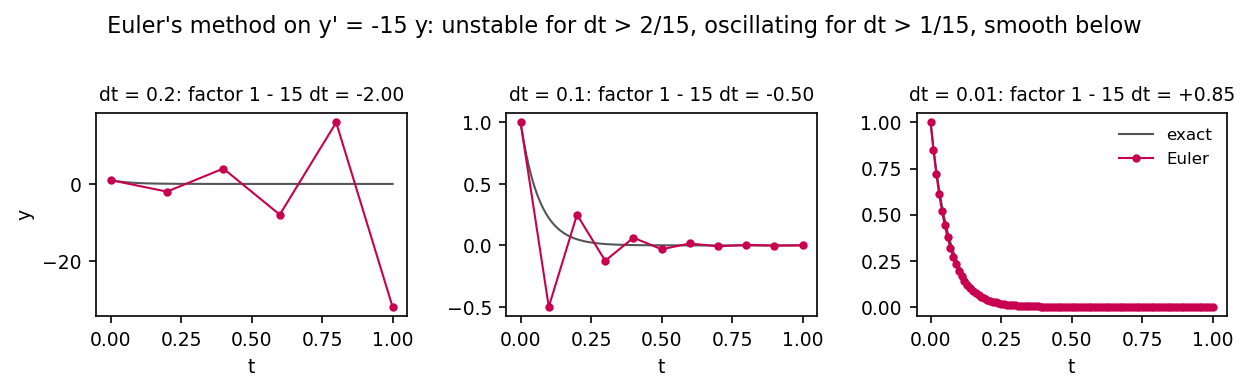
\includegraphics[width=\linewidth]{ch5-stiff-ode.png}
\end{column}
\begin{column}{0.52\textwidth}
\small Solve $y' = -15\,y$, $y(0) = 1$, whose exact solution $e^{-15t}$ decays smoothly, with Euler's method: $y_{n+1} = y_n + \Delta t\,(-15\,y_n) = (1 - 15\Delta t)\,y_n$.
\begin{itemize}
  \item Each step multiplies $y$ by $1 - 15\Delta t$. For $\Delta t = 0.2$ that factor is $-2$: the numerical solution \al{grows} and changes sign every step. Unstable.
  \item For $\Delta t = 0.1$ the factor is $-0.5$: it decays, but oscillates in sign. Stable, wrong in shape.
  \item For $\Delta t = 0.01$ the factor is $0.85$: smooth decay, close to the exact curve.
\end{itemize}
\begin{punchbox}
\small Stable for $\Delta t \le 2/15$, well-behaved for $\Delta t < 1/15$. The stiffer the equation (the larger the 15), the smaller the step. Springs in an IB model are exactly this kind of term.
\end{punchbox}
\end{column}
\end{columns}
\end{frame}

% 20
\begin{frame}[fragile]{Try it: the stiff equation}
\begin{columns}[T,onlytextwidth]
\begin{column}{0.5\textwidth}
In MATLAB or Octave, from \code{examples/support/matlab-exercises}:
\begin{lstlisting}[style=matlab]
stiff_ode_example(0.2, 1)    % unstable
stiff_ode_example(0.1, 1)    % stable, oscillates
stiff_ode_example(0.01, 1)   % smooth
\end{lstlisting}
In Python (the same plots, saved as \code{stiff\_ode\_example.png}; add \code{--show} for a window):
\begin{lstlisting}[style=shell]
python3 stiff_ode_example.py 0.2 1
python3 stiff_ode_example.py 0.1 1
python3 stiff_ode_example.py 0.01 1
\end{lstlisting}
\end{column}
\begin{column}{0.48\textwidth}
\begin{itemize}
  \item The arguments are the time step and the final time.
  \item Find the largest stable step by halving and doubling; then check the claim $\Delta t \le 2/15$ with $\Delta t = 0.13$ and $0.14$.
  \item Change $-15$ to $-150$ in the script. What happens to the stable step?
\end{itemize}
\begin{punchbox}
\small The scripts are the course's, with two bugs fixed: the MATLAB version allocated \code{zeros(N)} (an $N\times N$ matrix) instead of a vector and stopped one step before \code{tfinal}. The Python version writes the same numbers (Appendix A).
\end{punchbox}
\end{column}
\end{columns}
\end{frame}

% 21
\begin{frame}{Stability in a PDE: the heat equation}
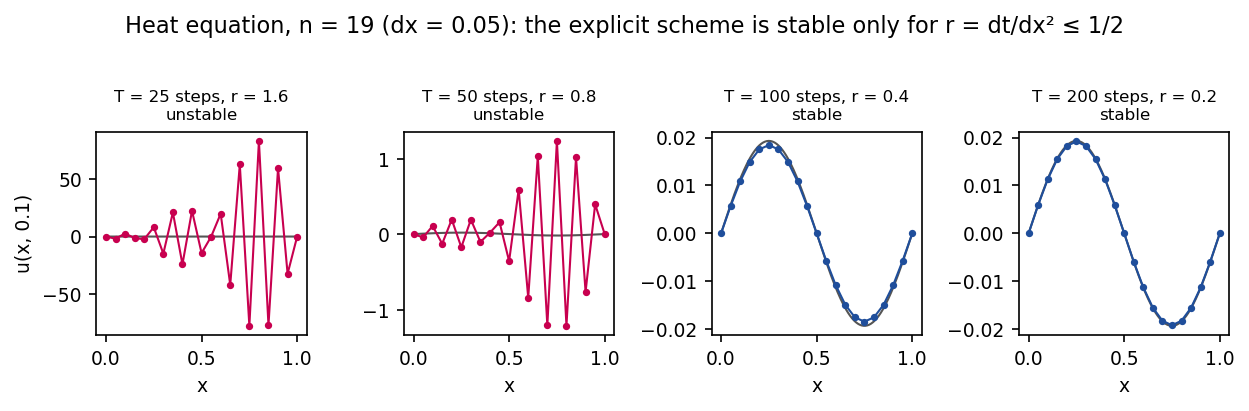
\includegraphics[width=\linewidth]{ch5-heat-time.png}
\vspace{1mm}

\small $u_t = u_{xx}$ on $0 < x < 1$ with $u = 0$ at the ends and $u(x,0) = \sin 2\pi x$: the temperature of a bar with a hot and a cold spot, which diffuse away. Exact solution $e^{-4\pi^2 t}\sin 2\pi x$. The explicit scheme $u_j^{n+1} = u_j^n + r\,(u_{j+1}^n - 2u_j^n + u_{j-1}^n)$ with $r = \Delta t/\Delta x^2$ is stable only for \al{$r \le 1/2$}.
\end{frame}

% 21b
\begin{frame}{The heat equation: what the four panels show}
\begin{itemize}
  \item With $n = 19$ interior points ($\Delta x = 0.05$) and $T$ steps to $t = 0.1$: $T = 25$ and $50$ ($r = 1.6$ and $0.8$) blow up (to about $10^{2}$ and $10^{0}$ by $t = 0.1$, and without bound after that), while $T = 100$ and $200$ ($r = 0.4$ and $0.2$) follow the exact curve.
  \item The growing mode is the most oscillatory one the grid can hold, $(-1)^j$, which is amplified by $|1 - 4r|$ per step: $5.4$ at $r = 1.6$, $2.2$ at $r = 0.8$. That is the zigzag in the unstable panels.
  \item Just above $r = 1/2$ the growth starts from rounding error and takes many steps to show: with $T = 70$ ($r = 0.57$) nothing is visible yet at $t = 0.1$. Instability is exponential, but it needs time.
  \item Halving $\Delta x$ forces $\Delta t$ down by four: the price of an explicit diffusion step, and the reason IBAMR treats viscosity implicitly.
\end{itemize}
\vspace{2mm}
\begin{punchbox}
\small An IB run that blows up does the same thing on its own grid: a short-wavelength mode in the structure or the velocity grows by a fixed factor per step until the numbers overflow, and a smaller step is the only cure.
\end{punchbox}
\end{frame}

% 22
\begin{frame}{Convergence in space}
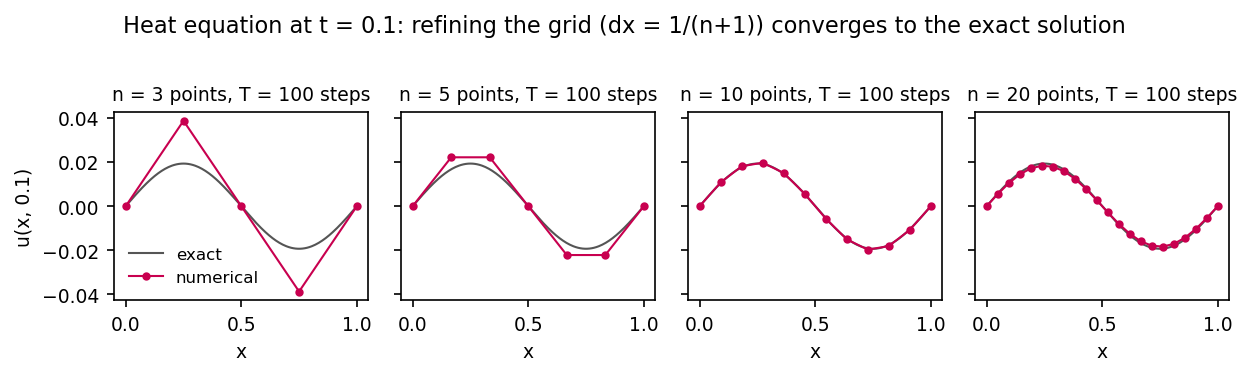
\includegraphics[width=\linewidth]{ch5-heat-space.png}
\vspace{1mm}

\small With $T = 100$ steps (always stable here) and $n = 3, 5, 10, 20$ points, the numerical solution approaches the exact curve: \al{convergence in space}. The scheme is second order in $\Delta x$: doubling $n$ divides the error by about 4. Measure it yourself: the error at $x = 1/4$ for $n = 5, 10, 20$.
\end{frame}

% 22b
\begin{frame}{Convergence in space: what it means for an IB run}
\begin{itemize}
  \item For an IB simulation the question is the same: is the flow around the boundary resolved? Are the shed vortices resolved? Is the gap between two structures resolved?
  \item Chapter 16 makes this a procedure: run on two or three grids ($N$, $2N$, $4N$ on the coarsest level, which refines every level), compare a number you care about (a drag force, a swimming speed, a tip position), and stop refining when it changes by less than you can accept.
  \item Convergence in time is checked the same way with $\Delta t$; in IB runs it is usually the space resolution that limits accuracy, because the time step is already small for stability (slide 27).
  \item Chapter 4d does the whole exercise in IB2d on a desktop PC, where a grid study takes minutes; the same study in IBAMR is the first thing to do before a long 3D run.
\end{itemize}
\vspace{2mm}
\begin{punchbox}
\small A converged answer on a coarse grid is worth more than an unconverged one on a fine grid, because you know what it means.
\end{punchbox}
\end{frame}

% 23
\begin{frame}[fragile]{Try it: the heat equation}
\begin{columns}[T,onlytextwidth]
\begin{column}{0.5\textwidth}
\begin{lstlisting}[style=matlab,basicstyle=\ttfamily\tiny\color{BlackGray}]
heat_equation(n, T)   % n interior points, T steps to t = 0.1
heat_equation(3, 100), heat_equation(5, 100)
heat_equation(10, 100), heat_equation(20, 100)  % space
heat_equation(19, 25), heat_equation(19, 50)    % unstable
heat_equation(19, 100), heat_equation(19, 200)  % stable
\end{lstlisting}
\begin{lstlisting}[style=shell,basicstyle=\ttfamily\tiny\color{BlackGray}]
python3 heat_equation.py 19 100   # dx = 0.05, r = 0.4
python3 heat_equation.py 19 50    # r = 0.8: blows up
python3 heat_equation.py 19 70    # r = 0.57: not yet visible
\end{lstlisting}
\end{column}
\begin{column}{0.48\textwidth}
\footnotesize
\begin{itemize}
  \item The plot shows the numerical and the exact solution at $t = 0.1$; the Python version prints the largest error, writes $\Delta x$, $\Delta t$ and $r$ on the plot and saves \code{heat\_equation.png}.
  \item The 2018 lecture used $n = 10$ with $T = 2, 4, 8, 16, 32, 64$. With so few points the unstable runs (any $T < 25$) have not yet grown visibly by $t = 0.1$, and the solutions look merely wrong; $n = 19$ with $T = 25$ and $50$ shows the real blow-up.
  \item The course's \code{heat\_equation.m} had a header that said $\sin 3\pi x$ while the code used $\sin 2\pi x$, and writes an EPS file on every call (\code{print -deps Example4\_1.eps}, left as it was: chapter 4d); the header is fixed, and the Python version gives the same numbers in the stable cases (checked with Octave; in the unstable ones the round-off that starts the blow-up differs from program to program, Appendix A).
\end{itemize}
\end{column}
\end{columns}
\end{frame}

% 24
\begin{frame}{Rate and order of convergence}
\begin{columns}[T,onlytextwidth]
\begin{column}{0.55\textwidth}
\small For a sequence $x_k \to L$:
\begin{itemize}
  \item it converges \al{linearly} if $|x_{k+1} - L| \le \mu\,|x_k - L|$ for some $0 < \mu < 1$; $\mu$ is the rate;
  \item it converges with \al{order $q > 1$} if $|x_{k+1} - L| \le C\,|x_k - L|^q$: quadratic for $q = 2$, cubic for $q = 3$ (Newton's method is quadratic).
\end{itemize}
For a discretization with step $h$ the error behaves like $E(h) \approx C h^p$, and $p$ is the \al{order of accuracy}. From two runs,
\[
p \approx \frac{\log\big(E(h_1)/E(h_2)\big)}{\log(h_1/h_2)} ,
\]
and when the exact solution is unknown, three runs with $h$, $h/2$, $h/4$ give $p$ from the differences between successive solutions.
\end{column}
\begin{column}{0.43\textwidth}
\begin{punchbox}
\small Chapter 16 does this with IBAMR: the same example on grids with $N$, $2N$ and $4N$ cells, a drag force or a tip position measured in each, and $p$ from the formula. Expect $p$ between 1 and 2 for an immersed boundary (next slide).
\end{punchbox}
\end{column}
\end{columns}
\end{frame}

% 25
\begin{frame}{How accurate is the IB method?}
\begin{columns}[T,onlytextwidth]
\begin{column}{0.55\textwidth}
\begin{itemize}
  \item The older lectures said ``second order in space if the boundary is smooth, first order if it has edges''. That is too generous.
  \item The fluid solver and the time stepping are second order, and the method is \al{formally second order} when everything is smooth, for example a smooth body force with no interface.
  \item But a thin elastic boundary makes the \al{pressure jump} and the \al{velocity gradient jump} across it, and the regularized delta function smears those jumps over a few cells. Near the boundary the error is then \al{first order} in $\Delta x$ (Griffith and Peskin 2005); away from it, second order.
\end{itemize}
\end{column}
\begin{column}{0.43\textwidth}
\begin{punchbox}
\small So: refine until the quantity you care about stops changing, and say on what grid it was computed. Do not expect halving $\Delta x$ to divide the error by four near an immersed boundary.
\end{punchbox}
\end{column}
\end{columns}
\end{frame}

% 25b
\begin{frame}{Accuracy in practice}
\begin{itemize}
  \item In practice the numbers you report (forces, speeds, positions) converge at a rate between 1 and 2, and the resolution of boundary layers and shed vortices matters more than the formal order.
  \item Quantities that live on the structure (a tip position, a swimming speed) converge faster than quantities that need the jump across it (the pressure difference across a membrane, the local shear stress), because the smearing of the kernel averages the latter over a few cells.
  \item The same holds for IBFE: the solid's interior is second order, but the fluid--solid interface is smeared in the same way (Griffith and Luo 2017 discuss the trade-offs).
  \item When you compare with an experiment or a body-fitted code, compare integrated quantities first (drag, lift, flow rate), then fields away from the boundary, and only last the fields at the boundary.
\end{itemize}
\vspace{2mm}
\small B. E. Griffith and C. S. Peskin, \emph{On the order of accuracy of the immersed boundary method: higher order convergence rates for sufficiently smooth problems}, J.\ Comput.\ Phys.\ 208 (2005) 75--105. B. E. Griffith and X. Luo, \emph{Hybrid finite difference/finite element immersed boundary method}, Int.\ J.\ Numer.\ Meth.\ Biomed.\ Engng 33 (2017) e2888.
\end{frame}

% 26
\begin{frame}{Time stepping in IBAMR}
\begin{itemize}
  \item The IB coupling (\code{IBExplicitHierarchyIntegrator}) uses the \al{midpoint rule} by default: forces and velocities are evaluated at $t + \Delta t/2$, which is second order in time. The trapezoidal rule is the other option.
  \item The fluid (\code{INSStaggeredHierarchyIntegrator}) uses a staggered-grid projection method: viscosity implicit, the convective term explicit with \al{Adams--Bashforth} (second order) and the \al{PPM} limiter, as in our inputs: \code{CONVECTIVE\_TS\_TYPE = "ADAMS\_BASHFORTH"}, \code{CONVECTIVE\_OP\_TYPE = "PPM"} (alternatives: \code{CUI}, \code{CENTERED}, \code{UPWIND}, \code{STABILIZED\_PPM}).
  \item The pressure is found by a projection: the velocity is advanced without the pressure gradient and then corrected so that $\nabla\cdot\mathbf{u} = 0$; the residuals of that solve are the \code{stokes solve} lines in the log (chapter 3).
\end{itemize}
\vspace{2mm}
\begin{punchbox}
\small The older notes said ``first or second order in time, depending on the version''. With IBAMR 0.16 and 0.19 and these inputs it is second order. The explicit coupling is also why the time step is limited by the stiffest force in the model (next slides).
\end{punchbox}
\end{frame}

% 26b
\begin{frame}{Time stepping in IBAMR: the first step, and the alternatives}
\begin{itemize}
  \item The first step has no history for Adams--Bashforth, so the integrator takes two cycles of fixed-point iteration; that is the message \code{attempting to perform 2 cycles of fixed point iteration} at the start of every run, and the reason a predictor--corrector advection--diffusion solver needs \code{init\_convective\_time\_stepping\_type = "FORWARD\_EULER"} (IBFE/12's README).
  \item A restarted run also starts with two cycles; the skip of the time-step-change check on the first step and after a restart is in the same place in the source (\code{IBHierarchyIntegrator.cpp}).
  \item \code{num\_cycles} in the integrator block asks for more cycles per step at every step; the course inputs use 1, and the examples here keep it.
  \item IBAMR also has implicit and semi-implicit IB integrators for very stiff structures, and a collocated-grid fluid solver (\code{SOLVER\_TYPE = "COLLOCATED"} in our inputs switches to it); chapter 15 looks at the examples that use them, and chapter 23 walks through the integrator calls in a main file.
\end{itemize}
\end{frame}

% 27
\begin{frame}{What limits the time step: the measured facts}
\scriptsize
\begin{tabular}{@{}L{0.15\textwidth}L{0.28\textwidth}L{0.09\textwidth}L{0.12\textwidth}L{0.23\textwidth}@{}}
\toprule
Example & Stiffest element & $\Delta x$ (m) & Largest \code{DT} that runs (s) & What the next larger step does\\
\midrule
IB/01 rubber band & springs $K/\Delta s = 2.0\times10^6$ & 1/512 & $5\times10^{-4}$ & $10^{-3}$ aborts within a few steps\\
IB/03 tethered leaf & beams $5.3\times10^6$, targets $3.1\times10^4$ & 1/512 & $2\times10^{-4}$ & $5\times10^{-4}$ aborts after 7 steps\\
IB/07 moving plates & targets $2.0\times10^6$ on every point & 1/512 & $10^{-4}$ & $2\times10^{-4}$ aborts after 7 steps\\
IB/04 bristles & targets $4.1\times10^6$ on every point & 1/1024 & $2\times10^{-5}$ & $5\times10^{-5}$ aborts after 22 steps\\
IB/08 glycocalyx (3D) & targets $3.2\times10^4$ on 13,600 points & 1/512 & $2\times10^{-5}$ & $5\times10^{-5}$: velocity grows tenfold per step, aborts after 4\\
IB/06 growing springs & springs $2.0\times10^6$ & 1/512 & $2\times10^{-4}$ & $5\times10^{-4}$ aborts after 136 steps\\
\bottomrule
\end{tabular}
\vspace{2mm}
\begin{itemize}
  \item The older lecture said ``the time step is inversely proportional to the force''. The measurements say it more usefully: \al{the stiffest element sets the step}, and \al{a finer grid needs a smaller step} too (the bristles, with stiffness scaled by $\Delta s$, need a step five times smaller on a grid twice as fine).
  \item For a single explicit spring of stiffness $\kappa$ on a mass $m$ the stable step is $\Delta t < 2\sqrt{m/\kappa}$; in a viscous fluid the drag changes the constant but not the trend: stiffer, smaller.
  \item None of these runs is anywhere near the CFL limit (next slide): the instability comes from the forcing, as the older lecture said.
\end{itemize}
\end{frame}

% 28
\begin{frame}[fragile]{What the blow-up looks like, and the keys behind it}
\begin{columns}[T,onlytextwidth]
\begin{column}{0.55\textwidth}
\begin{lstlisting}
IBHierarchyIntegrator::preprocessIntegrateHierarchy():
  Time step size change encountered.
Aborting.
\end{lstlisting}
\begin{itemize}
  \item Each step IBAMR computes the largest stable step from the velocities, $\Delta t_{\text{CFL}} = \code{cfl}\times\min(\Delta x/|u|)$ over all levels, and uses $\min(\code{dt\_max}, \Delta t_{\text{CFL}})$.
  \item While the run is healthy, $\Delta t_{\text{CFL}}$ is far larger than \code{dt\_max} and every step is \code{DT}. When the forcing instability makes the velocity grow, $\Delta t_{\text{CFL}}$ drops below \code{DT}, the step \emph{would} change, and with \code{error\_on\_dt\_change = TRUE} the IB integrator stops instead.
\end{itemize}
\end{column}
\begin{column}{0.43\textwidth}
\small Chapter 3 shows the same message in its table of first errors, with the rubber band at \code{DT = 1.0e-3}.
\end{column}
\end{columns}
\end{frame}

% 28c
\begin{frame}{The symptom and the cause}
\begin{itemize}
  \item So the message about the time step changing is the \al{symptom}; the cause is the stiff forcing. Lowering \code{cfl} or raising it changes nothing, because the CFL number was not the problem; what matters is the growth of the velocity near the structure.
  \item In 3D the same growth can trigger a regrid with absurd velocities first, and the run dies with \code{Internal RefineSchedule<DIM> error} instead (IB/08's README, at \code{DT = 5.0e-5}): the regrid asks for refinement where the exploding velocity is, in a place no coarser level covers.
  \item Both messages appear within a few steps of the start, or within a few steps of a change in the model (a stiffer spring, a faster target). A run that has gone on for thousands of steps and then stops with them has usually hit a new event: two structures meeting, a fold, a wall.
\end{itemize}
\vspace{2mm}
\begin{punchbox}
\small The fix is never to allow the change: it is a smaller \code{DT}, softer elements, or a slower motion. Chapter 16 gives the order in which to try them.
\end{punchbox}
\end{frame}

% 28b
\begin{frame}{The keys behind the time step}
\begin{columns}[T,onlytextwidth]
\begin{column}{0.5\textwidth}
\scriptsize
\begin{tabular}{@{}L{0.4\linewidth}L{0.52\linewidth}@{}}
\toprule
Key (our variable) & Meaning\\
\midrule
\code{dt\_max} (\code{DT}) & the step you ask for\\
\code{cfl} (\code{CFL\_MAX}, 0.3) & the CFL number allowed\\
\code{error\_on\_dt\_change} & abort when the step would change (TRUE here)\\
\code{warn\_on\_dt\_change} & warn instead of aborting\\
\code{grow\_dt} (\code{GROW\_DT}, 2) & how fast the step may grow after a reduction\\
\code{dt\_init}, \code{dt\_min} & the first step and the smallest allowed\\
\code{num\_cycles} & fixed-point cycles per step (1)\\
\code{regrid\_cfl\_interval} & regrid after this many cells of motion (0.5)\\
\bottomrule
\end{tabular}
\end{column}
\begin{column}{0.48\textwidth}
\small
\begin{itemize}
  \item \code{dt\_max} is the step you want; \code{DT} in our inputs is just the variable that feeds it (and \code{dt\_max} of the fluid integrator too).
  \item \code{cfl} is the CFL number the fluid integrator allows; 0.3 is the value in every example here.
  \item \code{grow\_dt} matters only when the step was reduced: it limits how fast the step may grow back. With \code{error\_on\_dt\_change = TRUE} a reduction never happens, so it is never used.
  \item \code{warn\_on\_dt\_change} instead of \code{error\_on\_dt\_change} lets the run continue with a smaller step; IBAMR's own examples do this, but a run that needs it is a run that is blowing up.
\end{itemize}
\end{column}
\end{columns}
\end{frame}

% 29
\begin{frame}{The CFL condition}
\begin{columns}[T,onlytextwidth]
\begin{column}{0.55\textwidth}
For an explicit scheme that transports something at speed $|u|$ on a grid with spacing $\Delta x$, information must not travel more than $C_{\max}$ cells per step:
\[
C = \frac{|u|\,\Delta t}{\Delta x} \le C_{\max}, \qquad\text{typically } C_{\max} \le 1 .
\]
\begin{itemize}
  \item Courant, Friedrichs and Lewy (1928): a necessary condition for the stability of explicit finite-difference schemes for hyperbolic equations; IBAMR's convective term is one.
  \item In IBAMR the check runs on every level, and the finest level is the binding one, since $\Delta x$ is smallest there.
\end{itemize}
\end{column}
\begin{column}{0.43\textwidth}
\begin{punchbox}
\small The condition says nothing about accuracy: a step that satisfies it can still be far too large for the stiff forces (slide 27). It is a floor under the step, not a recommendation.
\end{punchbox}
\end{column}
\end{columns}
\end{frame}

% 29b
\begin{frame}{The CFL condition in our runs}
\begin{itemize}
  \item In our runs $C$ is tiny: the rubber band at $0.1$ m/s with $\Delta t = 10^{-4}$ s and $\Delta x = 2$ mm gives $C = 0.005$. ``In IBAMR we rarely have to worry about the CFL condition'', as the older lecture said, is true for the runs in this series, \emph{until} something blows up (slide 28).
  \item When would it bind for real? Fast flows on fine grids: a prescribed motion at 1 m/s on a $1/1024$ m grid allows at most $\Delta t \approx 3\times10^{-4}$ s at \code{cfl = 0.3}, about the step the forcing allows anyway. Check it when you speed up a motion or refine the grid.
  \item The CFL number $C$ is also what \code{regrid\_cfl\_interval} counts (slide 32): the number of cells a point may have moved since the last regrid. With 0.5 and $C = 0.005$ per step, the rubber band regrids about every 100 steps, which matches the regrid lines in its log.
  \item The log prints the CFL number when logging is on; \code{grep -i cfl IB2d.log} shows it over the run, and a value that climbs toward 0.3 is the early warning of a blow-up.
\end{itemize}
\end{frame}

% 30
\begin{frame}{Resolution: what has to be resolved}
\begin{columns}[T,onlytextwidth]
\begin{column}{0.55\textwidth}
\footnotesize
\begin{itemize}
  \item The \al{boundary layer} on the structure: its thickness scales like $L/\sqrt{Re}$; at $Re = 2000$ and $L = 1$ that is about $0.02$, so a grid of $512$ cells across a box of width 2 puts about 5 cells in it. At $Re = 10^4$ it would be 2 cells.
  \item The \al{shed vortices}: a vortex needs several cells across its core, and it is advected for many steps, so a coarse grid both smears and misplaces it (chapter 1b's snake wake).
  \item The \al{gaps} between structures and the \al{thinnest features} of the structure itself: at least 4 to 8 cells (slide 16).
  \item The older notes said ``typically 512 $\times$ 512''. With adaptive refinement the finest level of our examples is 512 or 1024 cells across the box in 2D, and $64\times64\times512$ in 3D (IB/08), but only near the structure.
\end{itemize}
\end{column}
\begin{column}{0.43\textwidth}
\begin{punchbox}
\small The test is always the same: run on two grids and compare. If the number you care about changes by more than you can accept, refine again. Chapter 16 gives the procedure and the cost estimate; chapter 4d does it in IB2d, where it is cheap.
\end{punchbox}
\end{column}
\end{columns}
\end{frame}

% 31
\begin{frame}{Adaptive mesh refinement in IBAMR}
\begin{columns}[T,onlytextwidth]
\begin{column}{0.5\textwidth}
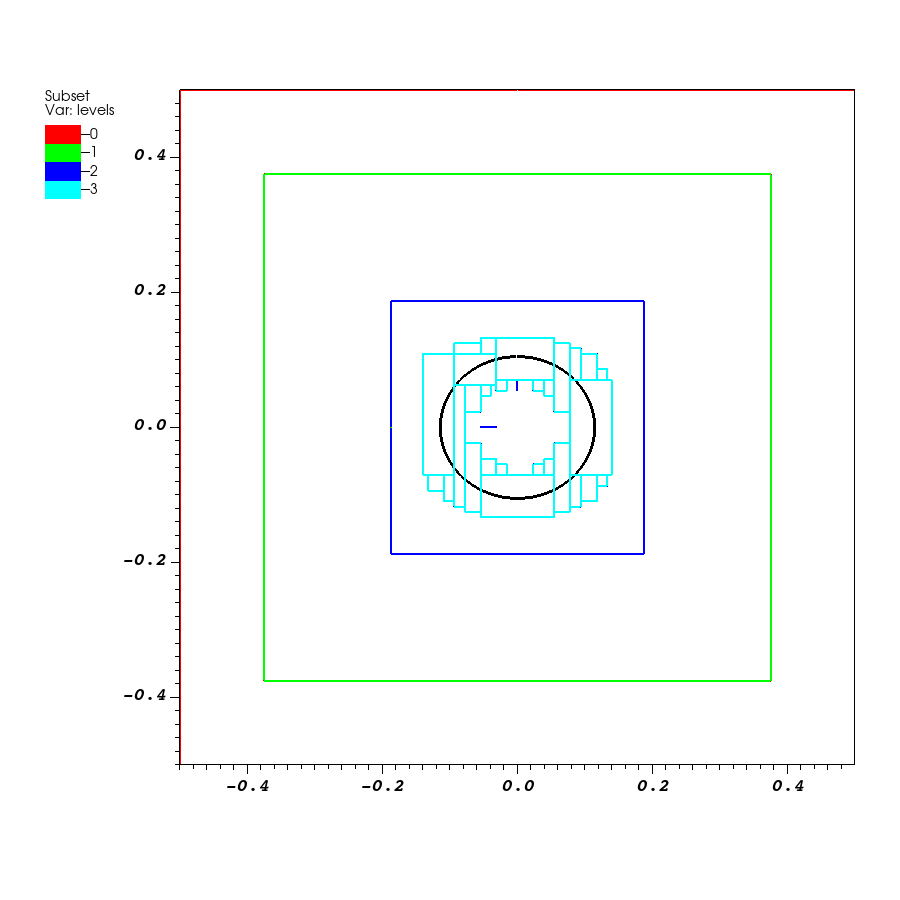
\includegraphics[width=0.84\linewidth]{ch5-rubber-band-levels.png}\\
{\tiny The rubber band's grid at $t = 0.12$ s: patch outlines of the four levels (example IB/01, IBAMR 0.19.0, rendered with VisIt).}
\end{column}
\begin{column}{0.48\textwidth}
\small
\begin{itemize}
  \item The domain is covered by a \al{hierarchy of levels}: level 0 is the coarsest grid ($N$ cells across); each finer level has cells \code{REF\_RATIO} times smaller (4 here) and covers only part of the domain, as a set of rectangular \al{patches}.
  \item Cells are \al{tagged} for refinement where the structure's points are, with \code{TAG\_BUFFER} extra cells around them, and optionally where the vorticity is large (\code{VORTICITY\_TAGGING}, \code{vorticity\_rel\_thresh}).
\end{itemize}
\end{column}
\end{columns}
\end{frame}

% 31b
\begin{frame}{Adaptive mesh refinement: where the structure lives and when the grid changes}
\begin{itemize}
  \item The structure always lives on the \al{finest} level (\code{level\_number = MAX\_LEVELS - 1} in the initializer block), so $\Delta x$ at the structure is $L/(N\cdot\code{REF\_RATIO}^{\code{MAX\_LEVELS}-1})$: $1/512$ m for the rubber band ($8\times4^3$) and for the leaf ($32\times4^2$), $1/1024$ m for the bristles ($16\times4^3$).
  \item The hierarchy is \al{regridded} when the points may have moved \code{regrid\_cfl\_interval} cells (0.5 here) or every \code{regrid\_interval} steps, so the fine patches follow the structure. The rubber band regridded 163 times in its 20,000 steps; the moving plates, which travel fastest, 413 times in 10,000.
  \item At a regrid the patches are rebuilt, the data copied, and the pressure re-projected (the \code{regridProjection} lines in the log); each regrid costs about as much as a few time steps.
  \item A structure given a \code{level\_number} that is not the finest, or that no longer exists after \code{MAX\_LEVELS} is changed, is the most common way to get a run that is silently wrong (slide 37).
\end{itemize}
\end{frame}

% 32
\begin{frame}{The basic adaptive IB approach, step by step}
\begin{columns}[T,onlytextwidth]
\begin{column}{0.5\textwidth}
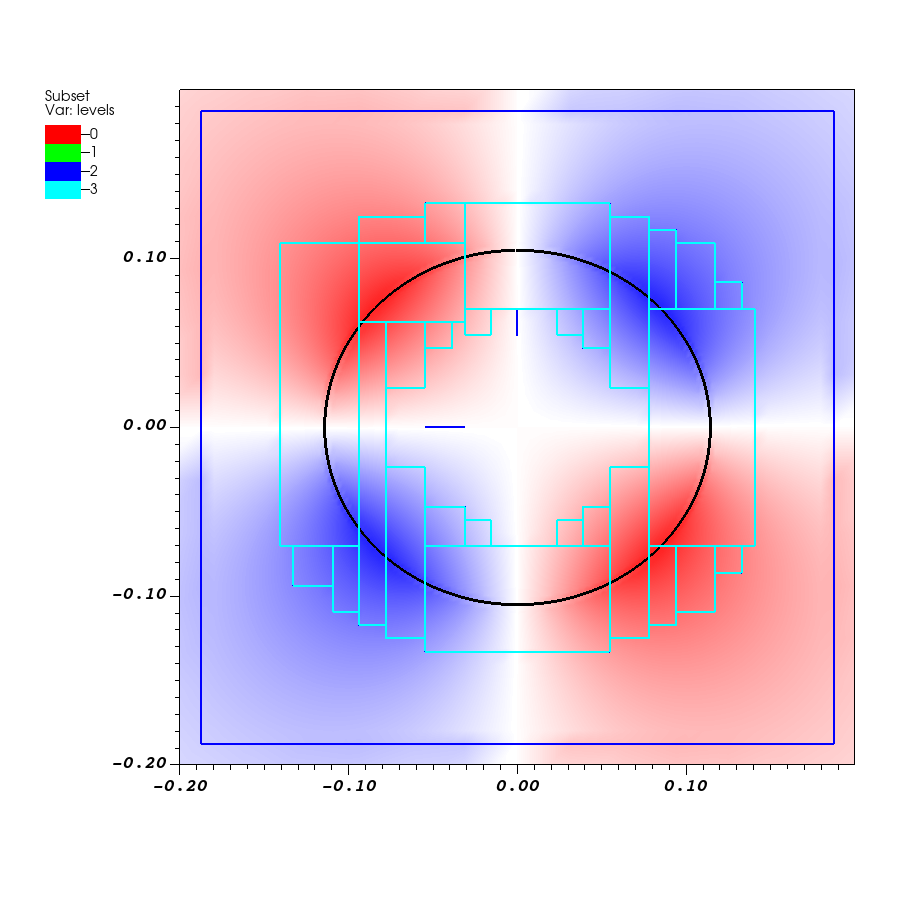
\includegraphics[width=0.84\linewidth]{ch5-rubber-band-amr.png}\\
{\tiny Vorticity of the relaxing rubber band with the patch outlines of the finest levels (IB/01, $t = 0.12$ s).}
\end{column}
\begin{column}{0.48\textwidth}
\small The five points of the 2014 lecture, which later versions dropped:
\begin{enumerate}
  \item Discretize the Eulerian equations on a Cartesian grid.
  \item \al{Refine the Cartesian grid near the boundary} (and where the flow needs it).
  \item Discretize the Lagrangian equations on a moving curvilinear mesh.
  \item The curvilinear mesh is \al{always at the same, finest, refinement level}: every point sees the same $\Delta x$, and the kernel never straddles a level boundary.
  \item Couple the two through regularized delta functions, as on a uniform grid.
\end{enumerate}
\end{column}
\end{columns}
\end{frame}

% 32b
\begin{frame}{What IBAMR adds to the method, and where these figures come from}
\begin{itemize}
  \item IBAMR is a parallel, adaptive implementation of exactly the method of slides 8--13; the adaptivity changes where the cells are, not what is done in them. The coupling, the kernel and the point spacing rules are those of the uniform-grid method.
  \item Because the structure is confined to the finest level, the delta function never has to be defined across a change of cell size; the coarser levels only carry the far field, and the finest level's cells are the $h$ of slides 12 and 13.
  \item Griffith, Hornung, McQueen and Peskin (2007) describe the adaptive method and show that it keeps the formal second-order accuracy of the uniform-grid scheme for smooth problems.
  \item The 2014--2025 lectures illustrated this with three figures from B. Griffith's 2009 MBI workshop slides (the link, \code{mbi.osu.edu/2009/ctwmaterials/griffith.pdf}, is dead). They are replaced here by renders of example IB/01 at $t = 0.12$ s with VisIt's Subset plot of the levels, which chapter 26 shows how to make.
\end{itemize}
\end{frame}

% 33
\begin{frame}{What adaptivity saves}
\begin{columns}[T,onlytextwidth]
\begin{column}{0.55\textwidth}
\scriptsize
\begin{tabular}{@{}L{0.18\linewidth}L{0.16\linewidth}L{0.2\linewidth}L{0.26\linewidth}@{}}
\toprule
Example & Levels, ratio & Finest grid if uniform & Cells in the hierarchy\\
\midrule
IB/01 rubber band & 4, ratio 4 (8 $\to$ 512) & $512^2 = 262{,}144$ & $16{,}528$ (16 times fewer): 64 + 576 + 2304 + 13,584 on levels 0 to 3\\
IB/03 tethered leaf & 3, ratio 4 (32 $\to$ 512) & $512^2 = 262{,}144$ & $4{,}608$ (57 times fewer): 1024 + 1024 + 2560\\
IB/08 glycocalyx (3D) & 3, ratio 4 & $64\times64\times512 = 2.1\times10^6$ & $161{,}280$ (13 times fewer)\\
\bottomrule
\end{tabular}
\vspace{1mm}
\footnotesize The counts come from the VisIt files of the runs described in the READMEs (the \code{summary.samrai} file of a dump lists every patch).
\end{column}
\begin{column}{0.43\textwidth}
\begin{punchbox}
\small VisIt's \textbf{Subset} plot of \code{levels} (chapter 26) shows you your own hierarchy; if the finest level covers most of the box, you are paying for a uniform grid with extra bookkeeping, and fewer levels would be faster.
\end{punchbox}
\end{column}
\end{columns}
\end{frame}

% 33b
\begin{frame}{What adaptivity costs}
\begin{itemize}
  \item The work per step is roughly proportional to the number of cells (plus the cost of the structure and of the solver's iterations), so a hierarchy with a tenth of the cells of the uniform fine grid is about ten times faster.
  \item The saving grows with the dimension and with how little of the box the structure occupies: that is why 3D is affordable at all. The glycocalyx run (IB/08) would take 13 times longer on a uniform $64\times64\times512$ grid.
  \item The price: regridding costs time (every regrid rebuilds the patches, copies the data and re-projects the pressure), and the fine patches must stay ahead of the structure, which is what \code{regrid\_cfl\_interval} and \code{tag\_buffer} arrange.
  \item The far field is computed on coarse cells: a vortex that leaves the refined region is smeared when it crosses into the coarse level. If the wake matters, turn on vorticity tagging, or add a wide \code{tag\_buffer}, and check that the answer does not change (chapter 16).
\end{itemize}
\end{frame}

% 34
\begin{frame}{Running in parallel}
\begin{columns}[T,onlytextwidth]
\begin{column}{0.55\textwidth}
\begin{itemize}
  \item The patches are distributed over the MPI processes (\code{mpirun -np 4}); the \code{LoadBalancer} block decides how (\code{bin\_pack\_method = "SPATIAL"}).
  \item Each process holds the structure points that lie in its patches, plus ghost copies near the patch edges, which is why the force-spreading and velocity-interpolation loops in the update functions walk both local and ghost nodes (IB/04, IB/06, IB/07).
\end{itemize}
\end{column}
\begin{column}{0.43\textwidth}
\begin{punchbox}
\small The adaptive hierarchy and the parallel decomposition are both handled by SAMRAI underneath IBAMR; you choose the levels, the ratio and the patch sizes in the \code{GriddingAlgorithm} block and the number of processes on the command line, and IBAMR does the rest.
\end{punchbox}
\end{column}
\end{columns}
\end{frame}

% 34b
\begin{frame}{Running in parallel: output, restarts and how many cores}
\begin{itemize}
  \item The output is written per process (\code{visit\_number\_procs\_per\_file}), and a restart needs the same number of processes as the run that wrote the restart files (chapter 3 shows the error you get otherwise).
  \item Small problems do not scale: the rubber band runs at the same speed on 4 and on 8 cores (10.5 against 10.2 ms per step), because communication and the solver's fixed costs dominate. Chapter 3's ``How many cores?'' gives the rule of thumb: a few tens of thousands of cells per process.
  \item The \code{smallest\_patch\_size} in the gridding block (32 cells here) sets the smallest piece of work a process can be given; with 16,528 cells in the rubber band's hierarchy and 28 patches on the finest level, 4 processes already leave some idle part of the time.
  \item 3D runs scale better: IB/08's 161,280 cells on 4 cores took 0.05 s per step, and the flow tank's larger hierarchy would use 8 to 16 cores well. Chapter 12 returns to this with the 3D examples.
\end{itemize}
\end{frame}

% 35
\begin{frame}[fragile]{The input keys behind this chapter: the integrators}
\begin{lstlisting}[style=input,basicstyle=\ttfamily\scriptsize\color{BlackGray}]
IBHierarchyIntegrator {
   dt_max              = DT        // the time step
   grow_dt             = GROW_DT   // growth after a reduction
   num_cycles          = 1
   regrid_cfl_interval = 0.5       // regrid after 0.5 cell of motion
   error_on_dt_change  = TRUE      // abort instead of changing DT
   tag_buffer          = 1         // extra cells refined around points
}
IBMethod {
   delta_fcn = "IB_4"              // the kernel
}
INSStaggeredHierarchyIntegrator {
   cfl                           = 0.3
   dt_max                        = DT
   convective_time_stepping_type = "ADAMS_BASHFORTH"
   convective_op_type            = "PPM"
   using_vorticity_tagging       = FALSE
   vorticity_rel_thresh          = 0.25,0.125
}
\end{lstlisting}
\small The IB integrator owns the time step and the regridding; the fluid integrator owns the CFL check, the convective scheme and the vorticity tagging. Both get \code{dt\_max}, and they must agree.
\end{frame}

% 35b
\begin{frame}[fragile]{The input keys behind this chapter: the grid and the structure}
\begin{lstlisting}[style=input,basicstyle=\ttfamily\tiny\color{BlackGray}]
GriddingAlgorithm {
   max_levels = MAX_LEVELS         // 3 or 4 here
   ratio_to_coarser { level_1 = 4,4  level_2 = 4,4 ... }
   largest_patch_size  { level_0 = NFINEST, NFINEST }
   smallest_patch_size { level_0 = 32, 32 }
   efficiency_tolerance = 0.85e0
   combine_efficiency   = 0.85e0
}
StandardTagAndInitialize {
   tagging_method = "GRADIENT_DETECTOR"
}
IBStandardInitializer {
   max_levels = MAX_LEVELS
   structure_names = "rubber_band_512"
   rubber_band_512 { level_number = MAX_LEVELS - 1 }
}
\end{lstlisting}
\small
\begin{itemize}
  \item \code{efficiency\_tolerance}: a patch is accepted when at least 85\% of its cells are tagged; \code{combine\_efficiency}: when to split a patch into smaller ones. \code{smallest\_patch\_size} and \code{largest\_patch\_size} bound the patches.
  \item Chapter 3 explains the file's structure; chapter 7 the boundary-condition blocks; chapter 6 the structure files.
\end{itemize}
\end{frame}

% 36
\begin{frame}{Rules of thumb}
\scriptsize
\begin{tabular}{@{}L{0.26\textwidth}L{0.68\textwidth}@{}}
\toprule
Choice & Rule, and where it comes from\\
\midrule
Point spacing & $\Delta s \approx \Delta x/2$ on the finest level for IB; elements about $\Delta x$ across for IBFE (slide 17)\\
Kernel & \code{IB\_4}; wider only together with coarser point spacing (slide 15)\\
Thin features and gaps & at least 4 to 8 cells, or they do not exist for the fluid (slide 16)\\
Time step & start from the example's value; halve until the run is stable, then check that halving again changes nothing you care about (slides 27--28)\\
Stiffness & no stiffer than the physics needs: every factor of 4 in stiffness costs a factor of 2 in the time step\\
Grid & refine until the quantity of interest stops changing; report the grid (slides 22, 25, 30)\\
Levels & 3 or 4 levels with ratio 4; the finest level only around the structure and its wake (slides 31--33)\\
Box & large enough that the walls do not change the answer (chapter 7)\\
Before a long run & a short run with a few steps, then a look at the output in VisIt (chapter 26)\\
\bottomrule
\end{tabular}
\vspace{2mm}
\begin{punchbox}
\small Every rule here was a lesson from a run that went wrong. The examples' READMEs record the ones that went wrong on purpose, with IBAMR's exact messages.
\end{punchbox}
\end{frame}

% 37
\begin{frame}{What can go wrong}
\scriptsize
\begin{tabular}{@{}L{0.3\textwidth}L{0.64\textwidth}@{}}
\toprule
Symptom & Cause and what to do\\
\midrule
\code{Time step size change encountered} after a few steps & the forcing instability: smaller \code{DT}, softer springs, slower motion (slides 27--28)\\
\code{Internal RefineSchedule<DIM> error} after a few steps (3D) & the same instability, caught by a regrid first (IB/08)\\
Fluid leaks through the structure & points farther apart than $\Delta x/2$, or elements larger than $\Delta x$: regenerate the structure for the grid (slide 17)\\
Two close structures behave as one & they are within the kernel's width: a wider gap or a finer grid (slide 16)\\
The answer changes when you refine & not converged: refine again, or accept and state the grid (slides 22, 30)\\
Nothing moves, or forces look wrong, after changing \code{MAX\_LEVELS} & the structure is assigned to a level that no longer exists or is not the finest: check \code{level\_number} (slide 31)\\
Very slow steps, many regrids in the log & \code{regrid\_cfl\_interval} too small for a fast motion, or a finest level that covers the whole box (slide 33)\\
Small jitter of a point at rest & the kernel's grid dependence: a wider kernel (\code{IB\_6}) smooths it (slide 15)\\
\bottomrule
\end{tabular}
\vspace{1mm}
\small Chapter 16 is the full troubleshooting chapter, with the convergence test as its first tool.
\end{frame}

% 38
\begin{frame}{Summary}
\begin{enumerate}
  \item An IB simulation solves the Navier--Stokes equations on a fixed grid with a force $\mathbf{f}$ from an elastic structure, and moves the structure with the fluid; the two are coupled by regularized delta functions that spread forces and interpolate velocities with the same kernel.
  \item The kernel is a few cells wide, so points should be about $\Delta x/2$ apart and nothing thinner than about 4 cells exists for the fluid.
  \item Convergence, order and stability: the two demo scripts show each; the IB method is first order near a thin boundary, so refine until the answer stops changing.
  \item The time step is limited by the stiffest element, not by the CFL condition; the limit shows up as ``Time step size change encountered''.
  \item IBAMR refines the grid only around the structure, keeps the structure on the finest level, and regrids as it moves; the keys are in the integrator, gridding and initializer blocks.
\end{enumerate}
\vspace{2mm}
\begin{homebox}
\small Next, chapter 6: the structure files (\code{.vertex}, \code{.spring}, \code{.beam}, \code{.target} and the rest), and the generators that write them.
\end{homebox}
\end{frame}

% 39
\begin{frame}{What changed since the older course notes}
\small
\begin{itemize}
  \item The accuracy statement is corrected: first order near a thin interface, second order for smooth problems (Griffith and Peskin 2005), instead of ``second order if smooth boundaries''.
  \item The time-step discussion is rebuilt from measurements on the examples (slide 27) and from IBAMR's actual logic: \code{cfl}, \code{dt\_max}, \code{error\_on\_dt\_change}, and why the CFL message is the symptom of a forcing instability.
  \item ``Two points per grid cell'' is kept for IB and stated in element sizes for IBFE, with the numbers of the examples and of IBAMR's own \code{ex4}.
  \item The time stepping is second order with these versions (midpoint rule, Adams--Bashforth), not ``first or second depending on the version''.
  \item The five AMR bullets of the 2014 UNC edition, dropped from the 2020 lecture, are back (slide 32).
  \item The equation images are typeset; B. Griffith's 2009 MBI figures (the link is dead) are replaced by renders of example IB/01; the four opening photographs are replaced by a table; IBAMR's kernel list comes from the 0.19.0 source.
  \item The demo scripts have Python versions and their bugs are fixed (Appendix A); the ``style.visibility'' residue and the Sakai download links are gone.
\end{itemize}
\end{frame}

% 40
\begin{frame}{References}
\scriptsize
\begin{itemize}
  \item C. S. Peskin. The immersed boundary method. \emph{Acta Numerica} 11:479--517, 2002.
  \item B. E. Griffith and C. S. Peskin. On the order of accuracy of the immersed boundary method: higher order convergence rates for sufficiently smooth problems. \emph{J.\ Comput.\ Phys.} 208:75--105, 2005.
  \item B. E. Griffith, R. D. Hornung, D. M. McQueen and C. S. Peskin. An adaptive, formally second order accurate version of the immersed boundary method. \emph{J.\ Comput.\ Phys.} 223:10--49, 2007.
  \item Y. Bao, J. Kaye and C. S. Peskin. A Gaussian-like immersed-boundary kernel with three continuous derivatives and improved translational invariance. \emph{J.\ Comput.\ Phys.} 316:139--144, 2016.
  \item B. E. Griffith and N. A. Patankar. Immersed methods for fluid--structure interaction. \emph{Annu.\ Rev.\ Fluid Mech.} 52:421--448, 2020 (open access: PMC7531444).
  \item N. A. Battista, W. C. Strickland and L. A. Miller. IB2d: a Python and MATLAB implementation of the immersed boundary method. \emph{Bioinspiration \& Biomimetics} 12:036003, 2017.
  \item R. Courant, K. Friedrichs and H. Lewy. \"Uber die partiellen Differenzengleichungen der mathematischen Physik. \emph{Math.\ Ann.} 100:32--74, 1928.
  \item IBAMR: \url{https://ibamr.github.io}; SAMRAI: \url{https://computing.llnl.gov/projects/samrai}. Kernel names: \code{ibtk/src/lagrangian/LEInteractor.cpp}; time-step logic: \code{src/IB/IBHierarchyIntegrator.cpp} and \code{src/navier\_stokes/INSHierarchyIntegrator.cpp}, IBAMR 0.19.0.
  \item \emph{Fluid Dynamics and IBM Theory}, modules 0-1, 0-2, 1-1, 1-2, 1-3, 1-4: \url{https://github.com/fairyflies9/Fluid-Dynamics-and-IBM-Theory}.
  \item Sources: \emph{0-IBAMR Tutorial: UNC Edition} (May 2014); \emph{Overview of IBM and Numerical Considerations} (MATH 769, January 2018; IBAMR lecture 2, 2020); \emph{Intro to IBM} (2025); the \code{stiff\_ode\_example} and \code{heat\_equation} scripts of the courses.
\end{itemize}
\end{frame}

\end{document}
